\section{Krylov子空间法}
\label{sec:ls-krylov-iterations}

定常迭代每轮施加同一个更新，前面算出的残差用过即弃。Krylov子空间法把这些残差及其矩阵乘积张成的子空间保留下来，每轮在逐步扩大的子空间中重新选择近似。本节先研究非奇异方阵：对称正定矩阵上的共轭梯度法，一般方阵上的Arnoldi正交化与GMRES，对称不定矩阵上的MINRES，以及非对称矩阵上保持短递推的BiCG与BiCGSTAB；再通过Golub--Kahan双对角化进入允许长方矩阵和秩亏的LSQR与LSMR。各方法分别说明它对矩阵的要求和它最小化的量。这些方法每轮的系数随当前向量变化，迭代不是同一个线性映射的反复作用，所以第~\ref{sec:ls-convergence}节关于固定误差矩阵的判据不能直接套用。Arnoldi正交化和Golub--Kahan双对角化只作为求解器内部生成基的过程介绍。

\subsection{Krylov子空间}
\label{sec:ls-krylov-subspaces}

设$\bm A\in\mathbb R^{d\times d}$。从初值$\bm x_0$出发，先算残差$\bm r_0=\bm b-\bm A\bm x_0$，它是修正方向最自然的起点；再反复乘以$\bm A$，得到第$k$个Krylov子空间
\[
 \mathcal K_k(\bm A,\bm r_0)=\operatorname{span}\{\bm r_0,\bm A\bm r_0,\ldots,\bm A^{k-1}\bm r_0\},
\]
不引起混淆时简写为$\mathcal K_k$。Krylov子空间法把第$k$步的候选解限制在仿射集合$\bm x_0+\mathcal K_k$中。每个新向量由上一个向量再乘一次$\bm A$得到，扩大子空间只需一次矩阵乘向量，不必形成矩阵的幂。

候选解与残差之间有一个多项式对应，后面各方法的收敛分析都从它出发。

\begin{lemma}[Krylov残差多项式]
\label{lem:ls-krylov-residual-polynomial}
记$\mathcal P_k=\{p:\deg p\le k,\ p(0)=1\}$。若$\bm x_k\in\bm x_0+\mathcal K_k$，则存在$p_k\in\mathcal P_k$使
\begin{equation}
 \label{eq:ls-krylov-residual-polynomial}
 \bm r_k=\bm b-\bm A\bm x_k=p_k(\bm A)\bm r_0 ;
\end{equation}
反之，对每个$p_k\in\mathcal P_k$，都有$\bm x_0+\mathcal K_k$中的一个候选，其残差为$p_k(\bm A)\bm r_0$。
\end{lemma}

\begin{proof}
$\bm x_k-\bm x_0$是$\bm r_0,\ldots,\bm A^{k-1}\bm r_0$的线性组合，可写成$q_{k-1}(\bm A)\bm r_0$，其中$\deg q_{k-1}\le k-1$。于是$\bm r_k=\bm r_0-\bm A\,q_{k-1}(\bm A)\bm r_0=p_k(\bm A)\bm r_0$，$p_k(t)=1-t\,q_{k-1}(t)\in\mathcal P_k$。反过来，$p_k\in\mathcal P_k$时$1-p_k(t)$在$t=0$处为零，可写成$t\,q_{k-1}(t)$，取$\bm x=\bm x_0+q_{k-1}(\bm A)\bm r_0$即可。
\end{proof}

于是选一个候选解就是选一个残差多项式。这个多项式由方法逐步选择：CG使误差的$\bm A$范数最小，GMRES使原残差的长度最小，BiCG则通过左右两组方向的配对确定近似。多项式随步数整体改变，不是某个固定更新矩阵的幂，所以收敛性要从各方法的选择准则推出，不能用固定更新矩阵的谱半径判断。

子空间随$k$嵌套增大，$\mathcal K_k\subseteq\mathcal K_{k+1}$，已有方向可以继续使用，新的一步在更大的候选集合中改进旧近似。但原始幂向量不宜直接作基：若$\bm A$有按模严格最大的特征值，$\bm A^j\bm r_0$的方向随$j$增大趋向相应的特征向量，相邻向量越来越接近平行，以它们为列的矩阵越来越病态。因此后面的方法要么显式正交化，要么利用矩阵结构得到有数学依据的短递推。精确算术下$\mathcal K_k$的维数不超过$d$，一旦不再扩张，它就是$\bm A$的不变子空间；但某个方法能否在有限步内求得精确解，还要结合它的选解准则和前提，不能只由维数上限推出。

对长方矩阵$\bm A\in\mathbb R^{m\times d}$，残差$\bm r_0\in\mathbb R^m$与未知量所在的$\mathbb R^d$维数不同，$\bm A\bm r_0$没有意义。第~\ref{sec:ls-bidiagonal-iteration}节的Golub--Kahan双对角化取零初值，在未知量空间中生成$\mathcal K_k(\bm A^\top\bm A,\bm A^\top\bm b)$的标准正交基，同时在数据空间中生成与之配对的基；计算时交替作用$\bm A$与$\bm A^\top$，不形成$\bm A^\top\bm A$。

\subsection{共轭梯度法}
\label{sec:ls-conjugate-gradient}

\subsubsection{主要思想}

设$\bm A=\bm A^\top\succ0$。正定性给出与问题相配的内积$\langle\bm u,\bm v\rangle_{\bm A}=\bm u^\top\bm A\bm v$及范数$\lVert\bm u\rVert_{\bm A}=(\bm u^\top\bm A\bm u)^{1/2}$。误差$\bm x-\bm x_\star$无法直接算出，但它的$\bm A$范数可以借一个能计算的二次函数来比较。令$\phi(\bm x)=\tfrac12\bm x^\top\bm A\bm x-\bm b^\top\bm x$，代入$\bm b=\bm A\bm x_\star$配方，得
\[
 \phi(\bm x)-\phi(\bm x_\star)=\tfrac12\lVert\bm x-\bm x_\star\rVert_{\bm A}^2 .
\]
所以在任何候选集合中，使$\phi$最小就是使误差的$\bm A$范数最小。从当前点$\bm x$沿方向$\bm p$走$\alpha$，记$\bm r=\bm b-\bm A\bm x$，则$\phi(\bm x+\alpha\bm p)=\phi(\bm x)-\alpha\,\bm p^\top\bm r+\tfrac12\alpha^2\,\bm p^\top\bm A\bm p$。这个一元二次式在$\alpha=\bm p^\top\bm r/(\bm p^\top\bm A\bm p)$处取最小值，这就是下面所用的步长。

逐个方向最小化时，后一步可能破坏前一步已经达到的最优。共轭梯度法（conjugate gradient method，CG）让搜索方向两两关于$\bm A$共轭，即$\bm p_i^\top\bm A\bm p_j=0$（$i\ne j$）。这时各方向对误差$\bm A$范数的贡献互不耦合，依次作一维最小化，就等于在全部方向张成的子空间上一次完成最小化。更重要的是，新方向只需由新残差加上最近一个旧方向的倍数得到，与更早方向的共轭关系自动成立，所以每轮只保存固定数量的向量。

\subsubsection{算法实现}

\paragraph{输入与初始化}
输入为对称正定矩阵$\bm A$和右端$\bm b$，算法只需要计算$\bm A$乘向量；超参数为初值$\bm x_0$、绝对与相对容差$\mathrm{atol},\mathrm{rtol}$及步数上限$K$，输出为近似解$\bm x$。停止沿用第~\ref{sec:ls-stationary-stopping}节的公共准则：$\lVert\bm r_k\rVert_2\le\mathrm{atol}+\mathrm{rtol}\lVert\bm b\rVert_2$时以达到要求结束，步数达到$K$时停止计算，两种情况都输出当前近似。初始化时计算$\bm r_0=\bm b-\bm A\bm x_0$，取第一个方向$\bm p_0=\bm r_0$；若初值已满足准则或$K=0$，直接输出$\bm x_0$。

\paragraph{沿当前方向更新}
第$k$轮先作本轮唯一的矩阵乘向量$\bm q_k=\bm A\bm p_k$，再计算步长，并沿$\bm p_k$更新解和残差：
\[
 \begin{gathered}
 \alpha_k=\frac{\bm r_k^\top\bm r_k}{\bm p_k^\top\bm q_k},\\
 \bm x_{k+1}=\bm x_k+\alpha_k\bm p_k,\qquad
 \bm r_{k+1}=\bm r_k-\alpha_k\bm q_k .
 \end{gathered}
\]
分子用$\bm r_k^\top\bm r_k$代替$\bm p_k^\top\bm r_k$，两者在精确算术下相等（见下面定理的证明），前者可以复用上一轮的内积。正定性保证非零方向上的分母$\bm p_k^\top\bm q_k>0$。残差借$\bm q_k$递推更新，不再另乘一次$\bm A$。

\paragraph{停止检验与新方向}
然后检验新残差。满足公共准则或$k+1=K$时输出$\bm x_{k+1}$；否则计算
\[
 \beta_k=\frac{\bm r_{k+1}^\top\bm r_{k+1}}{\bm r_k^\top\bm r_k},\qquad
 \bm p_{k+1}=\bm r_{k+1}+\beta_k\bm p_k,
\]
进入下一轮。检验放在形成新方向之前，残差为零时先结束，不再计算组合系数。

\begin{example}[CG在贯穿例上的两步]
\label{ex:ls-cg-two-steps}
取例~\ref{ex:ls-stationary-running-example}的$\bm A$、$\bm b=(1,2)^\top$与$\bm x_0=\bm 0$，其中$\bm A$的行为$(4,1)$与$(1,3)$。初始化得$\bm r_0=\bm p_0=(1,2)^\top$，$\bm r_0^\top\bm r_0=5$。第一轮$\bm q_0=\bm A\bm p_0=(6,7)^\top$，$\alpha_0=5/20=1/4$，于是$\bm x_1=(1/4,1/2)^\top$，$\bm r_1=\bm r_0-\alpha_0\bm q_0=(-1/2,1/4)^\top$；再由$\bm r_1^\top\bm r_1=5/16$得$\beta_0=1/16$，$\bm p_1=\bm r_1+\bm p_0/16=(-7/16,3/8)^\top$。可以核对$\bm r_1^\top\bm r_0=0$，$\bm p_1^\top\bm A\bm p_0=\bm p_1^\top\bm q_0=0$。

第二轮$\bm q_1=\bm A\bm p_1=(-11/8,11/16)^\top$，$\bm p_1^\top\bm q_1=55/64$，$\alpha_1=(5/16)/(55/64)=4/11$，得$\bm x_2=\bm x_1+\alpha_1\bm p_1=(1/11,7/11)^\top=\bm x_\star$，$\bm r_2=\bm 0$，两步即得精确解。若每轮都取$\beta_k=0$，即沿当前残差作精确一维最小化（最速下降），第一步与CG相同，此后在互相垂直的方向间折返，$\bm x_2=(1/12,7/12)^\top$、$\bm x_3=(5/48,5/8)^\top$，只能逐步逼近$\bm x_\star$。图~\ref{fig:ls-cg-steepest-descent-paths}把两条路径画在$\phi$的等值线上。
\end{example}

\begin{figure}[htbp]
  \centering
  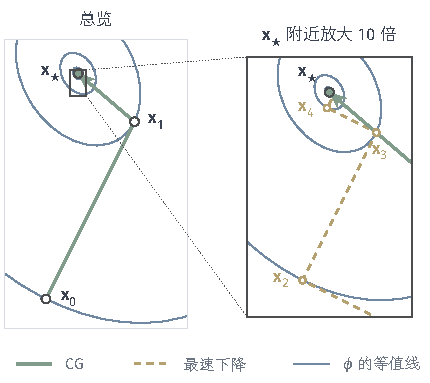
\includegraphics[width=72.873mm]{figures/01-basic-mathematics/03-vectors-matrices-and-multivariate-functions/tikz/c5-cg-steepest-descent-paths/figure.pdf}
  \caption{贯穿例上CG与最速下降的路径。蓝色椭圆是$\phi(\bm x)=\tfrac12\bm x^\top\bm A\bm x-\bm b^\top\bm x$经过最速下降各迭代点的等值线，中心为$\bm x_\star=(1/11,7/11)^\top$。两种方法的第一步都从$\bm x_0=\bm 0$走到$\bm x_1=(1/4,1/2)^\top$；CG的第二个方向与第一个方向$\bm A$共轭，直接指向椭圆中心，最速下降则在$\bm x_\star$附近来回折返（右图为左图小框放大10倍）。}
  \label{fig:ls-cg-steepest-descent-paths}
\end{figure}

\subsubsection{算法分析}

\paragraph{正确性与收敛速度}
正确性归结为两组关系：残差两两正交，方向两两共轭。由它们可以推出最优性，再由残差多项式得到收敛速度。

\begin{theorem}[CG的最优性与收敛速度]
\label{thm:ls-cg-convergence}
设$\bm A$对称正定，在精确算术下按上述递推计算，且$\bm r_0,\ldots,\bm r_{k-1}$均非零。则$\bm r_0,\ldots,\bm r_k$两两正交，$\bm p_0,\ldots,\bm p_{k-1}$两两关于$\bm A$共轭，$\bm x_k$是$\lVert\bm x-\bm x_\star\rVert_{\bm A}$在$\bm x_0+\mathcal K_k$上的唯一最小点，并且
\[
 \lVert\bm x_k-\bm x_\star\rVert_{\bm A}\le2\Bigl(\frac{\sqrt\kappa-1}{\sqrt\kappa+1}\Bigr)^k\lVert\bm x_0-\bm x_\star\rVert_{\bm A},
\]
其中$\kappa=\kappa_2(\bm A)$。CG至多$d$步得到精确解。
\end{theorem}

\begin{proof}
先归纳证明正交与共轭关系。设$\bm r_0,\ldots,\bm r_k$两两正交、$\bm p_0,\ldots,\bm p_k$两两共轭，且两组向量都张成$\mathcal K_{k+1}$；$k=0$时显然。由$\bm p_k=\bm r_k+\beta_{k-1}\bm p_{k-1}$及$\bm r_k\perp\bm p_{k-1}$，得$\bm p_k^\top\bm r_k=\bm r_k^\top\bm r_k$，于是步长的选法给出$\bm p_k^\top\bm r_{k+1}=0$；对$i<k$，$\bm p_i^\top\bm r_{k+1}=\bm p_i^\top\bm r_k-\alpha_k\bm p_i^\top\bm A\bm p_k=0$。所以$\bm r_{k+1}\perp\mathcal K_{k+1}$，特别与$\bm r_0,\ldots,\bm r_k$正交。对$i<k$，$\bm A\bm p_i\in\mathcal K_{i+2}\subseteq\mathcal K_{k+1}$，故$\bm r_{k+1}^\top\bm A\bm p_i=0$，从而$\bm p_{k+1}^\top\bm A\bm p_i=0$。对$i=k$，由$\bm A\bm p_k=(\bm r_k-\bm r_{k+1})/\alpha_k$得$\bm r_{k+1}^\top\bm A\bm p_k=-\bm r_{k+1}^\top\bm r_{k+1}/\alpha_k=-\beta_k\,\bm p_k^\top\bm A\bm p_k$，恰被$\beta_k$抵消。最后$\bm r_{k+1},\bm p_{k+1}\in\mathcal K_{k+2}$；若$\bm r_{k+1}\ne\bm 0$，正交的非零残差线性无关，两组向量都张成$\mathcal K_{k+2}$。

再证最优性。记$\bm e_k=\bm x_k-\bm x_\star$，则$\bm A\bm e_k=-\bm r_k$，且$\bm r_k\perp\mathcal K_k$。对任意$\bm z\in\mathcal K_k$，
\[
 \lVert\bm e_k+\bm z\rVert_{\bm A}^2
 =\lVert\bm e_k\rVert_{\bm A}^2-2\bm z^\top\bm r_k+\lVert\bm z\rVert_{\bm A}^2
 =\lVert\bm e_k\rVert_{\bm A}^2+\lVert\bm z\rVert_{\bm A}^2,
\]
所以$\bm x_k$是唯一最小点。$\mathbb R^d$中两两正交的非零向量至多$d$个，故至多$d$步出现零残差。

最后估计速度。按\eqref{eq:ls-krylov-residual-polynomial}的推导，$\bm x_0+\mathcal K_k$中候选的误差为$p(\bm A)\bm e_0$，其中$p$的次数不超过$k$且$p(0)=1$。由谱定理（定理~\ref{thm:ls-real-symmetric-spectral}）取标准正交特征向量展开$\bm e_0=\sum_ic_i\bm u_i$，得$\lVert p(\bm A)\bm e_0\rVert_{\bm A}^2=\sum_i\lambda_ip(\lambda_i)^2c_i^2\le\max_ip(\lambda_i)^2\,\lVert\bm e_0\rVert_{\bm A}^2$。取Chebyshev多项式$T_k$，它由$T_k(\cos\theta)=\cos k\theta$确定，在$[-1,1]$上$\lvert T_k\rvert\le1$；对$x>1$，$T_k(x)=\tfrac12[(x+\sqrt{x^2-1})^k+(x-\sqrt{x^2-1})^k]$，因为两边满足同一递推$T_{j+1}=2xT_j-T_{j-1}$和初值。令$\ell(t)=(\lambda_{\max}+\lambda_{\min}-2t)/(\lambda_{\max}-\lambda_{\min})$，它把$[\lambda_{\min},\lambda_{\max}]$映到$[-1,1]$，且$\ell(0)=(\kappa+1)/(\kappa-1)$。取$p(t)=T_k(\ell(t))/T_k(\ell(0))$，则在特征值上$\lvert p\rvert\le1/T_k(\ell(0))$。直接计算$x=\ell(0)$时$x+\sqrt{x^2-1}=(\sqrt\kappa+1)/(\sqrt\kappa-1)$，于是$T_k(\ell(0))\ge\tfrac12\bigl((\sqrt\kappa+1)/(\sqrt\kappa-1)\bigr)^k$，即得所述界。$\kappa=1$时$\bm A$是单位阵的倍数，一步得解。
\end{proof}

这个界只依赖两端特征值，误差缩小到给定比例所需的步数约与$\sqrt\kappa$成正比。它控制的是误差的$\bm A$范数，欧氏残差$\lVert\bm r_k\rVert_2$不必每步下降。

\paragraph{数值敏感度}
浮点计算中正交与共轭关系逐步受损，定理的有限步结论不能直接移用，实际计算不承诺恰好$d$步结束；递推残差也会偏离真实残差，所以宣布达到要求前按公共准则用$\bm b-\bm A\bm x_k$复核。

\paragraph{计算代价}
每轮核心递推需要一次$\bm A$乘向量、两次内积和三次向量更新。除矩阵外只保存$\bm x,\bm r,\bm p,\bm q$四个向量，存储不随步数增长；复核真实残差所需的矩阵乘向量另计。

\subsection{Arnoldi正交化}
\label{sec:ls-arnoldi}

\subsubsection{主要思想}

CG的短递推依赖对称正定结构。对一般非对称方阵，要在Krylov子空间中选解，先要有它的一组可靠的基。Arnoldi正交化不对病态的幂向量$\bm A^j\bm r_0$正交化，而把第~\ref{sec:ls-qr-method}节的修正Gram--Schmidt用于最新基向量的像$\bm A\bm v_j$：扣除它在已有基向量上的分量，剩余部分归一化后就是下一个基向量，扣除的系数记在一个小矩阵中。这样逐步得到$\mathcal K_k$的标准正交基。它是GMRES的内部步骤，所得的基与小矩阵不作为方程求解的输出。

\subsubsection{算法实现}

\paragraph{起始向量}
输入沿用GMRES的$\bm A,\bm b$和初值$\bm x_0$，生成的步数由GMRES的重启长度及总步数上限限定。先算$\bm r_0=\bm b-\bm A\bm x_0$；若它已满足公共停止准则，就不再生成基，否则令$\beta=\lVert\bm r_0\rVert_2$、$\bm v_1=\bm r_0/\beta$。

\paragraph{扣除已有分量}
第$j$轮先作一次矩阵乘向量$\bm w=\bm A\bm v_j$，再按$i=1,\ldots,j$依次计算
\[
 h_{i,j}=\bm v_i^\top\bm w,\qquad \bm w\leftarrow\bm w-h_{i,j}\bm v_i,
\]
每个系数都用已经扣除前面分量的当前$\bm w$计算。

\paragraph{归一化与提前终止}
扣除完毕后令$h_{j+1,j}=\lVert\bm w\rVert_2$，它衡量$\bm A\bm v_j$中有多少是新方向。若$h_{j+1,j}\ne0$，取$\bm v_{j+1}=\bm w/h_{j+1,j}$进入下一轮；若$h_{j+1,j}=0$，不再归一化，把本轮的系数交给GMRES完成当前的小问题。

\subsubsection{算法分析}

\paragraph{正确性}
把扣除的分量加回去，第$j$轮给出$\bm A\bm v_j=\sum_{i=1}^{j+1}h_{i,j}\bm v_i$。把各轮合成矩阵，就得到下面的Arnoldi关系，图~\ref{fig:ls-arnoldi-relation-shapes}画出了其中各矩阵的形状。

\begin{theorem}[Arnoldi关系]
\label{thm:ls-arnoldi-relation}
在精确算术下执行$k$轮Arnoldi正交化，且前$k-1$轮的$h_{j+1,j}$均非零。记$\bm V_k=[\bm v_1,\ldots,\bm v_k]\in\mathbb R^{d\times k}$，$\overline{\bm H}_k\in\mathbb R^{(k+1)\times k}$在$i\le j+1$处的元素为$h_{i,j}$、其余为零。若$h_{k+1,k}\ne0$，则$\bm v_1,\ldots,\bm v_{k+1}$标准正交，$\bm v_1,\ldots,\bm v_j$张成$\mathcal K_j$（$j\le k+1$），并且
\begin{equation}
 \label{eq:ls-arnoldi-relation}
 \bm A\bm V_k=\bm V_{k+1}\overline{\bm H}_k .
\end{equation}
若$h_{k+1,k}=0$，则$\bm v_1,\ldots,\bm v_k$标准正交且$\bm A\bm V_k=\bm V_k\bm H_k$，其中$\bm H_k$是$\overline{\bm H}_k$去掉末行所得的方阵，$\mathcal K_k$在$\bm A$下不变；$\bm A$非奇异时精确解$\bm x_\star$属于$\bm x_0+\mathcal K_k$。
\end{theorem}

\begin{proof}
关系式\eqref{eq:ls-arnoldi-relation}的第$j$列就是$\bm A\bm v_j=\sum_{i\le j+1}h_{i,j}\bm v_i$。对正交性归纳：设$\bm v_1,\ldots,\bm v_j$标准正交。第$i$次扣除后$\bm w\perp\bm v_i$，此后扣除的方向$\bm v_{i+1},\ldots,\bm v_j$都与$\bm v_i$正交，不破坏这一关系，所以最终的$\bm w$与$\bm v_1,\ldots,\bm v_j$都正交，归一化后得$\bm v_{j+1}$。又因$\bm A\bm v_j\in\mathcal K_{j+1}$，$\bm v_{j+1}\in\mathcal K_{j+1}$，$j+1$个标准正交向量张成维数不超过$j+1$的$\mathcal K_{j+1}$。若$h_{k+1,k}=0$，第$k$列成为$\bm A\bm v_k=\sum_{i\le k}h_{i,k}\bm v_i$，于是$\bm A\bm V_k=\bm V_k\bm H_k$，$\bm A\mathcal K_k\subseteq\mathcal K_k$。$\bm A$非奇异时它在有限维空间$\mathcal K_k$上是单射，因而也是满射；$\bm r_0\in\mathcal K_k$，故有$\bm z\in\mathcal K_k$使$\bm A\bm z=\bm r_0$，$\bm x_\star=\bm x_0+\bm z$。
\end{proof}

\begin{figure}[htbp]
  \centering
  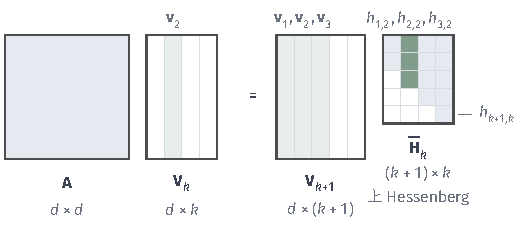
\includegraphics[width=89.098mm]{figures/01-basic-mathematics/03-vectors-matrices-and-multivariate-functions/tikz/c5-arnoldi-relation-shapes/figure.pdf}
  \caption{Arnoldi关系$\bm A\bm V_k=\bm V_{k+1}\overline{\bm H}_k$中各矩阵的形状（示意$d=7$、$k=4$）。$\overline{\bm H}_k$的非零元（浅蓝）只出现在主对角线、其上方和紧邻的下次对角线上，是上Hessenberg矩阵，末行只剩$h_{k+1,k}$。绿色标出第$j=2$列：$\bm A\bm v_2$只用到$\bm v_1,\bm v_2,\bm v_3$，系数是$\overline{\bm H}_k$第2列的前三个元素。}
  \label{fig:ls-arnoldi-relation-shapes}
\end{figure}

图中$\bm V_{k+1}$只比$\bm V_k$多一列，而$\overline{\bm H}_k$只有$k+1$行：$d$维的矩阵作用被压缩成一个小矩阵，GMRES与MINRES正是在这个小矩阵上求解。最后一种情形说明子空间不再扩张时，精确解已在候选集合中，GMRES在这一步得到精确解。

\paragraph{数值敏感度与计算代价}
有限精度下基的正交性会逐渐损失，判断与补救办法沿用第~\ref{sec:ls-qr-method}节对修正Gram--Schmidt的讨论。每轮新增一次$\bm A$乘向量。第$j$轮的投影约需$4dj$次浮点运算，$k$轮合计约$2dk^2$次；保存$\bm V_{k+1}$约需$(k+1)d$个数。投影工作量和基的存储都随保留的向量数增长；本过程只负责生成候选空间，收敛快慢由后面的选解方法决定。

\subsection{广义最小残差法}
\label{sec:ls-gmres}

\subsubsection{主要思想}

广义最小残差法（generalized minimal residual method，GMRES）在当前仿射Krylov空间中直接使原残差最小。设当前重启周期的起点为$\bm x^{(s)}$，残差为$\bm r^{(s)}$，$\beta=\lVert\bm r^{(s)}\rVert_2$，Arnoldi从$\bm v_1=\bm r^{(s)}/\beta$出发。写$\bm x=\bm x^{(s)}+\bm V_j\bm y$，由$\bm r^{(s)}=\beta\bm V_{j+1}\bm e_1$及\eqref{eq:ls-arnoldi-relation}，
\[
 \bm b-\bm A\bm x=\bm r^{(s)}-\bm A\bm V_j\bm y=\bm V_{j+1}(\beta\bm e_1-\overline{\bm H}_j\bm y).
\]
$\bm V_{j+1}$的列标准正交，乘以它不改变长度，于是$d$维中的最小化化为$(j+1)\times j$的小型最小二乘问题
\[
 \min_{\bm y\in\mathbb R^j}\lVert\beta\bm e_1-\overline{\bm H}_j\bm y\rVert_2 .
\]
它用第~\ref{sec:ls-qr-method}节的Givens旋转化为上三角，再调用回代求解。$\overline{\bm H}_j$每列只在对角线下多一个非零元，所以每增加一列只需一次新旋转，前面的旋转可以保留下来重复使用。

\subsubsection{算法实现}

\paragraph{输入与初始化}
输入为非奇异方阵$\bm A$与$\bm b$；超参数为$\bm x_0,\mathrm{atol},\mathrm{rtol},K$和重启长度$m$（$1\le m\le d$），输出为$\bm x$。初始化时令$\bm x^{(s)}=\bm x_0$，计算$\bm r^{(s)}=\bm b-\bm A\bm x^{(s)}$；若公共停止准则未满足，令$\beta=\lVert\bm r^{(s)}\rVert_2$、$\bm v_1=\bm r^{(s)}/\beta$，并把小问题的右端置为$\bm g=(\beta,0,\ldots,0)^\top$。

\paragraph{Arnoldi扩展}
每个内步$j$先按第~\ref{sec:ls-arnoldi}节作一轮Arnoldi，扩充所存的基，并得到$\overline{\bm H}_j$的新列$(h_{1,j},\ldots,h_{j+1,j})^\top$。

\paragraph{旋转更新残差}
然后用Givens旋转更新残差估计。前面各列已被保存的旋转$\bm G_1,\ldots,\bm G_{j-1}$化成上三角，新列也要依次经过这些旋转，整个矩阵才对应同一个正交变换。此后新列只剩两个待处理的元素：第$j$行的$a$和第$j+1$行的$h=h_{j+1,j}$。令
\[
 \begin{gathered}
 \rho_j=\sqrt{a^2+h^2},\qquad c_j=a/\rho_j,\qquad s_j=h/\rho_j,\\
 \bm G_j=\begin{bmatrix}c_j&s_j\\-s_j&c_j\end{bmatrix},
 \end{gathered}
\]
$\bm G_j$作用于第$j,j+1$行，把$(a,h)^\top$变为$(\rho_j,0)^\top$。同一旋转作用于右端，把$(g_j,0)^\top$变为$(c_jg_j,-s_jg_j)^\top$，即$g_j\leftarrow c_jg_j$、$g_{j+1}=-s_jg_j$，前面已确定的分量不变。旋转后前$j$行构成上三角矩阵$\bm R_j$，小问题的最小残差就是$\lvert g_{j+1}\rvert$，不必形成近似解即可判断是否停止。

\paragraph{回代、恢复解与重启}
最后一个环节是回代求系数并恢复解。当$\lvert g_{j+1}\rvert$满足阈值、Arnoldi不再生成新方向、本周期已达$m$步或总步数达到$K$时，结束内步，用回代解$\bm R_j\bm y=(g_1,\ldots,g_j)^\top$，并恢复$\bm x=\bm x^{(s)}+\bm V_j\bm y$。再用原矩阵计算$\bm b-\bm A\bm x$，按公共准则复核：满足阈值或已达总步数上限就输出$\bm x$；否则以该$\bm x$为新周期的起点$\bm x^{(s)}$，从它的残差重新生成基。Arnoldi给出$h_{j+1,j}=0$时，$s_j=0$且$g_{j+1}=0$，先完成小问题，不再用该系数作除法。

\begin{example}[GMRES在贯穿例上的两步]
\label{ex:ls-gmres-two-steps}
仍取例~\ref{ex:ls-stationary-running-example}的$\bm A,\bm b$与$\bm x_0=\bm 0$，$m=2$。初始化得$\beta=\sqrt5$，$\bm v_1=(1,2)^\top/\sqrt5$，$\bm g=(\sqrt5,0)^\top$。第一个内步$\bm A\bm v_1=(6,7)^\top/\sqrt5$，扣除得$h_{1,1}=4$、$\bm w=(2,-1)^\top/\sqrt5$，于是$h_{2,1}=1$，$\bm v_2=(2,-1)^\top/\sqrt5$。旋转取$\rho_1=\sqrt{17}$、$c_1=4/\sqrt{17}$、$s_1=1/\sqrt{17}$，右端变为$\bm g=(4\sqrt5,-\sqrt5)^\top/\sqrt{17}$，残差估计$\lvert g_2\rvert=\sqrt{5/17}\approx0.542$。若在此停止，回代得$y_1=g_1/\rho_1=4\sqrt5/17$，$\bm x_1=y_1\bm v_1=(4/17,8/17)^\top$；复核$\bm b-\bm A\bm x_1=(-7,6)^\top/17$，长度正是$\sqrt{5/17}$，小于CG第一步的残差长度$\sqrt5/4\approx0.559$。

第二个内步$\bm A\bm v_2=(7,-1)^\top/\sqrt5$，扣除得$h_{1,2}=1$、$h_{2,2}=3$，剩余向量为零，$h_{3,2}=0$，二维空间已经用尽。新列$(1,3,0)^\top$先经$\bm G_1$变为$(7,11,0)^\top/\sqrt{17}$，新旋转$c_2=1$、$s_2=0$，$g_3=0$。回代求解
\[
 \bm R_2\bm y=\frac1{\sqrt{17}}\begin{bmatrix}17&7\\0&11\end{bmatrix}\bm y
 =\frac{\sqrt5}{\sqrt{17}}\begin{bmatrix}4\\-1\end{bmatrix},
\]
得$y_2=-\sqrt5/11$、$y_1=3\sqrt5/11$，于是恢复出$\bm x_2=y_1\bm v_1+y_2\bm v_2=(1/11,\,7/11)^\top$，正是$\bm x_\star$。
\end{example}

\subsubsection{算法分析}

\paragraph{正确性}
下面的定理针对不重启的完整GMRES，即$m=d$的情形。

\begin{theorem}[GMRES的最小残差性]
\label{thm:ls-gmres-optimality}
设$\bm A$非奇异，在精确算术下执行完整GMRES的第$k$步，记$\bm r_k=\bm b-\bm A\bm x_k$。则$\bm x_k$是$\bm x_0+\mathcal K_k$中残差长度的唯一最小点，$\lVert\bm r_k\rVert_2=\lvert g_{k+1}\rvert$，它等于上一步的残差长度乘以$\lvert s_k\rvert\le1$，因而随$k$不增；GMRES至多$d$步得到精确解。若$\bm A=\bm X\bm\Lambda\bm X^{-1}$可对角化（$\bm X,\bm\Lambda$可以是复矩阵），还有
\[
 \lVert\bm r_k\rVert_2\le\kappa_2(\bm X)\min_{p\in\mathcal P_k}\max_{\lambda\in\sigma(\bm A)}\lvert p(\lambda)\rvert\,\lVert\bm r_0\rVert_2,
\]
其中$\mathcal P_k$同引理~\ref{lem:ls-krylov-residual-polynomial}。
\end{theorem}

\begin{proof}
Arnoldi尚未停止时$\bm V_k$满列秩，$\bm A$非奇异，所以$\bm A\bm V_k=\bm V_{k+1}\overline{\bm H}_k$满列秩，$\overline{\bm H}_k$也满列秩。映射$\bm y\mapsto\bm x_0+\bm V_k\bm y$是$\mathbb R^k$到$\bm x_0+\mathcal K_k$的双射，且由主要思想中的推导，两边的残差长度相等，所以两个最小化问题的解一一对应。记$k$个旋转之积为$\bm\Omega_k$，它是正交矩阵，满足$\bm\Omega_k\overline{\bm H}_k=\begin{bmatrix}\bm R_k\\\bm 0^\top\end{bmatrix}$、$\bm\Omega_k\beta\bm e_1=\bm g$，故
\[
 \lVert\beta\bm e_1-\overline{\bm H}_k\bm y\rVert_2^2
 =\lVert(g_1,\ldots,g_k)^\top-\bm R_k\bm y\rVert_2^2+g_{k+1}^2 .
\]
$\bm R_k$与$\overline{\bm H}_k$秩相同，可逆，回代所得的$\bm y$使第一项为零，且是唯一使之为零的点，最小值为$\lvert g_{k+1}\rvert$。第$k$个旋转把上一步的$g_k$变为$c_kg_k$与$-s_kg_k$，所以$\lvert g_{k+1}\rvert=\lvert s_k\rvert\,\lvert g_k\rvert$，其中$\lvert g_k\rvert$是旋转前的值，即上一步的残差长度。若$h_{k+1,k}=0$，则$\bm A\bm V_k=\bm V_k\bm H_k$，$\bm H_k$可逆，取$\bm y=\beta\bm H_k^{-1}\bm e_1$即得零残差；子空间维数不超过$d$，所以至多$d$步出现这一情形或零残差。最后，由引理~\ref{lem:ls-krylov-residual-polynomial}，$\lVert\bm r_k\rVert_2=\min_{p\in\mathcal P_k}\lVert p(\bm A)\bm r_0\rVert_2$；而$p(\bm A)=\bm Xp(\bm\Lambda)\bm X^{-1}$，对角矩阵$p(\bm\Lambda)$的谱范数是$\max_{\lambda\in\sigma(\bm A)}\lvert p(\lambda)\rvert$，乘上$\lVert\bm X\rVert_2\lVert\bm X^{-1}\rVert_2=\kappa_2(\bm X)$即得所述界。
\end{proof}

\paragraph{收敛速度}
定理中的界把收敛问题化为多项式逼近：要找在原点取值$1$、在全部特征值上都很小的低次多项式。非正规矩阵的$\kappa_2(\bm X)$可能很大，界因此变弱，只看特征值是否集中不能判断收敛快慢。

\paragraph{重启与数值敏感度}
重启的GMRES($m$)丢弃了历史空间，最优性只在一个周期内成立，可能停滞，也不再有$d$步得到精确解的保证。浮点计算中基不再精确正交，$\lvert g_{j+1}\rvert$与真实残差会偏离，这就是每个周期结束时用$\bm b-\bm A\bm x$复核的原因。

\paragraph{计算代价}
每个内步需要一次$\bm A$乘向量。完整GMRES执行$k$步时，正交化共约$2dk^2$次浮点运算，基的存储约$kd$个数，都随步数增长；GMRES($m$)把历史基限制在一个周期内，每周期至多约$2dm^2$次运算，存储约$(m+1)d$个数，与总步数无关。

\subsection{最小残差法}
\label{sec:ls-minres}

\subsubsection{主要思想}

若$\bm A$对称，Arnoldi得到的$\bm H_k=\bm V_k^\top\bm A\bm V_k$也对称；它又是上Hessenberg矩阵，因而是三对角矩阵，Arnoldi退化为Lanczos三项递推，每轮只需扣除两个方向。最小残差法（minimal residual method，MINRES）在这一递推上仍然在当前Krylov空间中最小化欧氏残差。它不要求正定，适用于对称不定矩阵；小问题的三角因子带宽固定，解也能用短递推更新，不必保存全部基。

\subsubsection{算法实现}

\paragraph{输入与初始化}
输入为实对称非奇异矩阵$\bm A$与$\bm b$，允许$\bm A$不定；超参数为$\bm x_0,\mathrm{atol},\mathrm{rtol},K$，输出为$\bm x$。先算$\bm r_0=\bm b-\bm A\bm x_0$并按公共准则检查；未结束时令$\beta=\lVert\bm r_0\rVert_2$，取$\bm v_0=\bm 0$、$\bm v_1=\bm r_0/\beta$、$\gamma_0=0$、$\bm d_{-1}=\bm d_0=\bm 0$、$\bar g_1=\beta$，并把两个尚不存在的旧旋转置为$(c_{-1},s_{-1})=(c_0,s_0)=(1,0)$。

\paragraph{Lanczos三项递推}
第$j$轮先作一步Lanczos递推：
\[
 \begin{gathered}
 \bm w=\bm A\bm v_j-\gamma_{j-1}\bm v_{j-1},\qquad a_j=\bm v_j^\top\bm w,\\
 \bm w\leftarrow\bm w-a_j\bm v_j,\qquad \gamma_j=\lVert\bm w\rVert_2 .
 \end{gathered}
\]
三对角矩阵的第$j$列因而为$(\gamma_{j-1},a_j,\gamma_j)^\top$，位于第$j-1,j,j+1$行。

\paragraph{旋转消元}
然后按GMRES的旋转约定处理这一列：第$j-2$个旋转作用于第$j-2,j-1$行的$(0,\gamma_{j-1})$，第$j-1$个旋转作用于所得的第二个分量与$a_j$，最后构造消去$\gamma_j$的新旋转：
\[
 \begin{gathered}
 \epsilon_j=s_{j-2}\gamma_{j-1},\qquad \theta=c_{j-2}\gamma_{j-1},\\
 \delta_j=c_{j-1}\theta+s_{j-1}a_j,\qquad
 \bar\delta=-s_{j-1}\theta+c_{j-1}a_j,\\
 \rho_j=\sqrt{\bar\delta^2+\gamma_j^2},\qquad
 c_j=\bar\delta/\rho_j,\qquad s_j=\gamma_j/\rho_j .
 \end{gathered}
\]
旋转后，三角因子的第$j$列只有$\epsilon_j,\delta_j,\rho_j$三个非零元，分别位于第$j-2,j-1,j$行。

\paragraph{更新解与停止}
最后更新右端、方向与解：
\[
 \begin{gathered}
 g_j=c_j\bar g_j,\qquad \bar g_{j+1}=-s_j\bar g_j,\\
 \bm d_j=\frac{\bm v_j-\delta_j\bm d_{j-1}-\epsilon_j\bm d_{j-2}}{\rho_j},\qquad
 \bm x_j=\bm x_{j-1}+g_j\bm d_j .
 \end{gathered}
\]
$\lvert\bar g_{j+1}\rvert$是当前残差长度的内部估计，用它按公共准则判断是否终止并输出$\bm x_j$。若$\gamma_j=0$，完成本轮的解更新后即结束；未结束时才令$\bm v_{j+1}=\bm w/\gamma_j$进入下一轮。非奇异条件保证正常步骤中$\rho_j>0$。

\subsubsection{算法分析}

\paragraph{正确性}
MINRES是GMRES在对称矩阵上的短递推实现，因而保留了GMRES的最小残差性。

\begin{theorem}[MINRES的最小残差性]
\label{thm:ls-minres-optimality}
设$\bm A$实对称非奇异，在精确算术下执行MINRES至第$k$步，且此前的$\gamma_1,\ldots,\gamma_{k-1}$均非零。则$\bm x_k$与完整GMRES的第$k$个近似相同，是残差长度在$\bm x_0+\mathcal K_k$上的唯一最小点；$\lVert\bm r_k\rVert_2=\lvert\bar g_{k+1}\rvert$随$k$不增，MINRES至多$d$步得到精确解，并且
\[
 \lVert\bm r_k\rVert_2\le\min_{p\in\mathcal P_k}\max_{\lambda\in\sigma(\bm A)}\lvert p(\lambda)\rvert\,\lVert\bm r_0\rVert_2 .
\]
\end{theorem}

\begin{proof}
由\eqref{eq:ls-arnoldi-relation}及$\bm V_k$的标准正交性，$\bm H_k=\bm V_k^\top\bm A\bm V_k$；$\bm A$对称时它也对称。上Hessenberg矩阵在主对角线下方只有一条非零次对角线，对称后上方也只有一条，所以$\bm H_k$是三对角矩阵，$h_{j-1,j}=h_{j,j-1}=\gamma_{j-1}$，Arnoldi的投影只剩Lanczos递推中的两项。于是$\bm A\bm V_k=\bm V_{k+1}\overline{\bm T}_k$，$\overline{\bm T}_k$是$(k+1)\times k$的三对角矩阵，上述旋转正是GMRES对它施加的旋转，所得上三角因子$\bm R_k$上带宽为$2$。令$\bm D_k=[\bm d_1,\ldots,\bm d_k]$满足$\bm D_k\bm R_k=\bm V_k$，比较第$j$列得$\bm v_j=\epsilon_j\bm d_{j-2}+\delta_j\bm d_{j-1}+\rho_j\bm d_j$，这就是方向递推。GMRES的解为$\bm x_k=\bm x_0+\bm V_k\bm R_k^{-1}(g_1,\ldots,g_k)^\top=\bm x_0+\bm D_k(g_1,\ldots,g_k)^\top$，而右端已确定的分量此后不再改变，所以逐步加上$g_j\bm d_j$得到的正是GMRES的近似。其余结论由定理~\ref{thm:ls-gmres-optimality}得到；对称矩阵可取正交的特征向量矩阵$\bm X$，$\kappa_2(\bm X)=1$。
\end{proof}

\paragraph{收敛速度}
界中只剩特征值，收敛快慢完全由谱决定。不定时特征值分布在原点两侧，而多项式在原点必须取$1$，要同时压低两侧谱上的值，比只压低一侧更难。

\paragraph{数值敏感度与计算代价}
浮点计算中Lanczos向量会失去正交性，残差估计须用真实残差复核；这里不扩展到奇异对称系统与MINRES-QLP。每轮核心递推需要一次$\bm A$乘向量，只保存$\bm v_{j-1},\bm v_j,\bm w,\bm d_{j-2},\bm d_{j-1},\bm x$等固定数量的向量；若为保持正交性作完整的再正交化，就要保存全部基，存储随步数增长。

\subsection{双共轭梯度法}
\label{sec:ls-bicg}

\subsubsection{主要思想}

非对称矩阵上，Arnoldi要对全部旧基向量投影，代价随步数增长。双共轭梯度法（biconjugate gradient method，BiCG）放弃残差最小化，改用$\bm A$与$\bm A^\top$同时生成两个序列：原序列位于$\mathcal K_k(\bm A,\bm r_0)$，影子序列位于$\mathcal K_k(\bm A^\top,\widetilde{\bm r}_0)$。它不再要求原残差彼此正交，而要求原残差与影子残差相互正交，即双正交。这个条件只用相邻两项的递推就能维持，形式与CG相同，但不需要CG的正定误差内积。

\subsubsection{算法实现}

\paragraph{输入与初始化}
输入为实非奇异方阵$\bm A$与$\bm b$，算法需要计算$\bm A$与$\bm A^\top$乘向量；超参数为$\bm x_0,\mathrm{atol},\mathrm{rtol},K$及影子初值$\widetilde{\bm r}_0$，输出为$\bm x$。先算$\bm r_0=\bm b-\bm A\bm x_0$并按公共准则检查；未结束时选取满足$\widetilde{\bm r}_0^\top\bm r_0\ne0$的影子初值，默认$\widetilde{\bm r}_0=\bm r_0$，再取$\bm p_0=\bm r_0$、$\widetilde{\bm p}_0=\widetilde{\bm r}_0$、$\rho_0=\widetilde{\bm r}_0^\top\bm r_0$。

\paragraph{两个序列同步更新}
第$k$轮先计算$\bm q_k=\bm A\bm p_k$和$\widetilde{\bm q}_k=\bm A^\top\widetilde{\bm p}_k$，再以$\alpha_k=\rho_k/(\widetilde{\bm p}_k^\top\bm q_k)$同时更新解和两个残差：
\[
 \begin{gathered}
 \bm x_{k+1}=\bm x_k+\alpha_k\bm p_k,\\
 \bm r_{k+1}=\bm r_k-\alpha_k\bm q_k,\qquad
 \widetilde{\bm r}_{k+1}=\widetilde{\bm r}_k-\alpha_k\widetilde{\bm q}_k .
 \end{gathered}
\]

\paragraph{停止检验与新方向}
然后按公共准则检验原残差与步数上限。未结束时计算$\rho_{k+1}=\widetilde{\bm r}_{k+1}^\top\bm r_{k+1}$、$\beta_k=\rho_{k+1}/\rho_k$，再取
\[
 \bm p_{k+1}=\bm r_{k+1}+\beta_k\bm p_k,\qquad
 \widetilde{\bm p}_{k+1}=\widetilde{\bm r}_{k+1}+\beta_k\widetilde{\bm p}_k .
\]
这些公式要求尚未结束时的配对分母$\rho_k$与$\widetilde{\bm p}_k^\top\bm A\bm p_k$非零。零残差先由停止检验结束；残差非零而配对量为零时递推中断，不再继续相除，也不能把它当作收敛。

\subsubsection{算法分析}

\paragraph{正确性}
BiCG选取近似的依据是下面的双正交关系，证明沿用CG的归纳，只是把每个内积的左因子换成影子序列。

\begin{theorem}[BiCG的双正交性]
\label{thm:ls-bicg-biorthogonality}
设在精确算术下BiCG执行到第$k$步，此前的$\rho_0,\ldots,\rho_k$与$\widetilde{\bm p}_i^\top\bm A\bm p_i$（$i<k$）均非零。则对$i,j\le k$、$i\ne j$，
\[
 \widetilde{\bm r}_i^\top\bm r_j=0,\qquad \widetilde{\bm p}_i^\top\bm A\bm p_j=0,
\]
并且$\bm r_k\perp\mathcal K_k(\bm A^\top,\widetilde{\bm r}_0)$。这个正交条件确定了BiCG在$\bm x_0+\mathcal K_k$中选取的近似。
\end{theorem}

\begin{proof}
对$k$归纳，设结论对$k$成立。由递推，$\bm p_i$与$\bm r_0,\ldots,\bm r_i$张成同一空间，$\widetilde{\bm p}_i$与$\widetilde{\bm r}_0,\ldots,\widetilde{\bm r}_i$亦然，故$\widetilde{\bm p}_i^\top\bm r_k=0$（$i<k$），从而$\widetilde{\bm p}_k^\top\bm r_k=\widetilde{\bm r}_k^\top\bm r_k=\rho_k$。步长$\alpha_k$因此使$\widetilde{\bm p}_k^\top\bm r_{k+1}=\rho_k-\alpha_k\widetilde{\bm p}_k^\top\bm A\bm p_k=0$；对$i<k$，$\widetilde{\bm p}_i^\top\bm r_{k+1}=\widetilde{\bm p}_i^\top\bm r_k-\alpha_k\widetilde{\bm p}_i^\top\bm A\bm p_k=0$。所以$\bm r_{k+1}$与$\widetilde{\bm r}_0,\ldots,\widetilde{\bm r}_k$都正交；把两个序列的角色互换，同理$\widetilde{\bm r}_{k+1}$与$\bm r_0,\ldots,\bm r_k$正交。

再看共轭。由$\bm A^\top\widetilde{\bm p}_i=(\widetilde{\bm r}_i-\widetilde{\bm r}_{i+1})/\alpha_i$，对$i<k$有$\widetilde{\bm p}_i^\top\bm A\bm r_{k+1}=0$，于是$\widetilde{\bm p}_i^\top\bm A\bm p_{k+1}=\widetilde{\bm p}_i^\top\bm A\bm r_{k+1}+\beta_k\widetilde{\bm p}_i^\top\bm A\bm p_k=0$。对$i=k$，$\widetilde{\bm p}_k^\top\bm A\bm r_{k+1}=-\rho_{k+1}/\alpha_k$，而$\beta_k\widetilde{\bm p}_k^\top\bm A\bm p_k=(\rho_{k+1}/\rho_k)(\rho_k/\alpha_k)=\rho_{k+1}/\alpha_k$，两者抵消。由$\bm A\bm p_i=(\bm r_i-\bm r_{i+1})/\alpha_i$，同理得$\widetilde{\bm p}_{k+1}^\top\bm A\bm p_i=0$（$i\le k$）。最后，$\rho_i\ne0$与双正交性给出$\widetilde{\bm r}_0,\ldots,\widetilde{\bm r}_{k-1}$线性无关：若$\sum_ic_i\widetilde{\bm r}_i=\bm 0$，与$\bm r_j$作内积得$c_j\rho_j=0$。它们都属于$\mathcal K_k(\bm A^\top,\widetilde{\bm r}_0)$，因而张成该空间，$\bm r_k$与之正交。
\end{proof}

\paragraph{收敛性与数值敏感度}
双正交条件不是某个范数的最小化，BiCG因而没有CG或GMRES那样的单调最小性，一般也不存在只靠$\kappa_2(\bm A)$就能承诺的统一下降速度。配对量很小时，除以它会放大已有的舍入误差，残差可能剧烈振荡，配对量为零时递推中断；这里保留这一限制，不展开中断的分类与修补策略。每轮需要一次$\bm A$乘向量和一次$\bm A^\top$乘向量，工作向量数量固定。

\subsection{稳定化双共轭梯度法}
\label{sec:ls-bicgstab}

\subsubsection{主要思想}

BiCG每轮需要$\bm A^\top$的作用，残差也可能剧烈振荡。稳定化双共轭梯度法（biconjugate gradient stabilized method，BiCGSTAB）只用一个固定的影子向量$\widehat{\bm r}$计算BiCG型递推所需的配对系数，不再生成影子序列。每轮先沿BiCG型方向走一步，得到中间残差；再沿$\bm A$作用于中间残差的方向作一次一元最小化，把残差压低。这样每轮只需要$\bm A$的作用。

\subsubsection{算法实现}

\paragraph{输入与初始化}
输入为实非奇异方阵$\bm A$与$\bm b$；超参数为$\bm x_0,\mathrm{atol},\mathrm{rtol},K$及固定的影子向量$\widehat{\bm r}$，输出为$\bm x$。下面的写法参照文献中的模板\scite{math-barrett1994templates}。先算$\bm r_0=\bm b-\bm A\bm x_0$并按公共准则检查；未结束时取满足$\widehat{\bm r}^\top\bm r_0\ne0$的影子向量，默认$\widehat{\bm r}=\bm r_0$。

\paragraph{形成搜索方向}
第$k$轮先算$\rho_k=\widehat{\bm r}^\top\bm r_k$，再形成搜索方向。首轮取$\bm p_0=\bm r_0$；以后各轮取
\[
 \beta_k=\frac{\rho_k}{\rho_{k-1}}\cdot\frac{\alpha_{k-1}}{\omega_{k-1}},\qquad
 \bm p_k=\bm r_k+\beta_k(\bm p_{k-1}-\omega_{k-1}\bm v_{k-1}).
\]

\paragraph{BiCG半步}
然后走第一个半步：
\[
 \bm v_k=\bm A\bm p_k,\qquad
 \alpha_k=\frac{\rho_k}{\widehat{\bm r}^\top\bm v_k},\qquad
 \bm s_k=\bm r_k-\alpha_k\bm v_k ,
\]
$\bm s_k$是中间近似$\bm x_k+\alpha_k\bm p_k$的残差。先用它检验中间近似：若满足公共准则，就输出$\bm x_k+\alpha_k\bm p_k$，不再走第二个半步。

\paragraph{残差最小化半步}
未结束时走第二个半步：
\[
 \begin{gathered}
 \bm t_k=\bm A\bm s_k,\qquad \omega_k=\frac{\bm t_k^\top\bm s_k}{\bm t_k^\top\bm t_k},\\
 \bm x_{k+1}=\bm x_k+\alpha_k\bm p_k+\omega_k\bm s_k,\qquad
 \bm r_{k+1}=\bm s_k-\omega_k\bm t_k ,
 \end{gathered}
\]
再按公共准则终止或进入下一轮。所用的配对分母$\rho_k$、$\widehat{\bm r}^\top\bm v_k$及下一轮要除的$\omega_k$都须非零。中间残差为零时已由前面的检验结束，避免在已求得解时计算$0/0$；其余中断情形不展开成异常清单。

\begin{example}[BiCGSTAB在贯穿例上的一轮]
\label{ex:ls-bicgstab-one-step}
仍取例~\ref{ex:ls-stationary-running-example}的$\bm A,\bm b$与$\bm x_0=\bm 0$，影子向量$\widehat{\bm r}=\bm r_0=(1,2)^\top$。首轮$\rho_0=5$，$\bm p_0=\bm r_0$。第一个半步$\bm v_0=\bm A\bm p_0=(6,7)^\top$，$\alpha_0=5/20=1/4$，$\bm s_0=(-1/2,1/4)^\top$，中间近似$(1/4,1/2)^\top$与CG第一步相同，$\lVert\bm s_0\rVert_2=\sqrt5/4\approx0.559$。第二个半步$\bm t_0=\bm A\bm s_0=(-7/4,1/4)^\top$，$\bm t_0^\top\bm s_0=15/16$，$\bm t_0^\top\bm t_0=50/16$，故$\omega_0=3/10$，于是
\[
 \begin{gathered}
 \bm x_1=(1/4,1/2)^\top+\tfrac3{10}\bm s_0=(1/10,23/40)^\top,\\
 \bm r_1=\bm s_0-\omega_0\bm t_0=(1/40,7/40)^\top .
 \end{gathered}
\]
直接计算$\bm b-\bm A\bm x_1$得到同一向量，$\lVert\bm r_1\rVert_2=\sqrt{50}/40\approx0.177$，比中间残差小了约三分之二。
\end{example}

\subsubsection{算法分析}

\paragraph{第二个半步的作用}
第二个半步的系数来自一个一元二次式。展开
\[
 \lVert\bm s_k-\omega\bm t_k\rVert_2^2=\lVert\bm s_k\rVert_2^2-2\omega\,\bm t_k^\top\bm s_k+\omega^2\lVert\bm t_k\rVert_2^2,
\]
它在$\omega=\omega_k$处取最小值$\lVert\bm s_k\rVert_2^2-(\bm t_k^\top\bm s_k)^2/\lVert\bm t_k\rVert_2^2$，所以$\lVert\bm r_{k+1}\rVert_2\le\lVert\bm s_k\rVert_2$。这只是相对于中间残差的局部改进：第一个半步可能使$\lVert\bm s_k\rVert_2$大于$\lVert\bm r_k\rVert_2$，因而不保证$\lVert\bm r_{k+1}\rVert_2\le\lVert\bm r_k\rVert_2$，也不保证在所有非奇异系统上收敛。收敛快慢取决于实际形成的残差多项式。

\paragraph{数值敏感度与计算代价}
影子配对量很小或$\omega_k$很小时，后续系数对舍入敏感，所以仍按公共准则复核原残差。完整一轮通常需要两次$\bm A$乘向量，使用固定数量的工作向量；在中间阶段终止时，只需要第一个半步的一次乘法。
